\documentclass[
	a4paper,
	oneside,
	DIV = 12,
	12pt,
	headings = normal,
]{scrartcl}

%%% Length calculations
\usepackage{calc}
%%%

%%% Support for color
\usepackage{xcolor}
\definecolor{lightblue}{HTML}{03A9F4}
\definecolor{red}{HTML}{F44336}
%%%

%%% Including graphics
\usepackage{graphicx}
%%%

%%% Font selection
\usepackage{fontspec}

\setromanfont{STIX Two Text}[
	SmallCapsFeatures = {LetterSpace = 5},
]

\setsansfont{IBM Plex Sans}[
	Scale = MatchUppercase,
]

\setmonofont{IBM Plex Mono}[
	Scale = MatchUppercase,
]
%%%

%%% Math typesetting
\usepackage{amsmath}

\usepackage{unicode-math}
\setmathfont{STIX Two Math}
%%%

%%% List settings
\usepackage{enumitem}
\setlist[enumerate]{
	label*      = {\arabic*.},
	leftmargin  = *,
	labelindent = \parindent,
	topsep      = 1\baselineskip,
	parsep      = 0\baselineskip,
	itemsep     = 1\baselineskip,
}

\setlist[itemize]{
	label*      = {—},
	leftmargin  = *,
	labelindent = \parindent,
	topsep      = 1\baselineskip,
	parsep      = 0\baselineskip,
	itemsep     = 1\baselineskip,
}

\setlist[description]{
	font        = {\rmfamily\upshape\bfseries},
	topsep      = 1\baselineskip,
	parsep      = 0\baselineskip,
	itemsep     = 0\baselineskip,
}

%%%

%%% Structural elements typesetting
\setkomafont{pagenumber}{\rmfamily}
\setkomafont{disposition}{\rmfamily\bfseries}

% Sectioning
\RedeclareSectionCommand[
	beforeskip = -1\baselineskip,
	afterskip  = 1\baselineskip,
	font       = {\normalsize\bfseries\scshape},
]{section}

\RedeclareSectionCommand[
	beforeskip = -1\baselineskip,
	afterskip  = 1\baselineskip,
	font       = {\normalsize\bfseries},
]{subsection}

\RedeclareSectionCommand[
	beforeskip = -1\baselineskip,
	afterskip  = 1\baselineskip,
	font       = {\normalsize\bfseries},
]{subsubsection}
%%%

%%% Typographic enhancements
\usepackage{microtype}
%%%

%%% Language-specific settings
\usepackage{polyglossia}
\setmainlanguage{ukrainian}
%%%

%%% Captions
\usepackage{caption}
\usepackage{subcaption}

%\DeclareCaptionLabelFormat{closing}{#2)}
%\captionsetup[subtable]{labelformat = closing}

%\captionsetup[subfigure]{labelformat = closing}

\captionsetup[table]{
	aboveskip = 0\baselineskip,
	belowskip = 1\baselineskip,
}

\captionsetup[figure]{
	aboveskip = 1\baselineskip,
	belowskip = 0\baselineskip,
}

\captionsetup[subfigure]{
	labelformat = simple,
	labelformat = brace,
}
%%%

%%% Table typesetting
\usepackage{booktabs}
\usepackage{longtable}

\usepackage{multirow}

\usepackage{array}
\newcolumntype{v}[1]{>{\raggedright\arraybackslash\hspace{0pt}}p{#1}}
\newcolumntype{b}[1]{>{\centering\arraybackslash\hspace{0pt}}p{#1}}
\newcolumntype{n}[1]{>{\raggedleft\arraybackslash\hspace{0pt}}p{#1}}
%%%

%%% Dingbats
\usepackage{pifont}
%%%

%%% Links and hyperreferences
\usepackage{hyperref}
\hypersetup{
	bookmarksnumbered = true,
	colorlinks      = false,
	linkbordercolor = red,
	urlbordercolor  = lightblue,
	pdfborderstyle  = {/S/U/W 1.5},
}
%%%

%%% Length adjustments
% Set baselineskip to ~15pt, default is 14.5pt
% \linespread{1.034483}
\linespread{1.068966} % ~15.5pt
\setlength{\emergencystretch}{1em}
\setlength{\parindent}{1.5em}
\newlength{\gridunitwidth}
\setlength{\gridunitwidth}{\textwidth / 12}
\setlength{\floatsep}{1\baselineskip}
\setlength{\intextsep}{1\baselineskip}
\setlength{\textfloatsep}{1\baselineskip}
%%%

%%% Custom commands
\newcommand{\allcaps}[1]{{\addfontfeatures{LetterSpace = 5}#1}}
\newcommand{\progname}[1]{\texttt{#1}}

\newcommand{\CheckMark}{\ding{51}}
%%%

\begin{document}
	\begin{titlepage}
		\begin{center}
			Міністерство освіти і науки України\\
			Національний авіаційний університет\\
			Навчально-науковий інститут комп'ютерних інформаційних технологій\\
			Кафедра комп'ютеризованих систем управління

			\vspace{\fill}
				Лабораторна робота №1.1\\
				з дисципліни «Системне програмне забезпечення»\\
				на тему «Ознайомлення з~програмним забезпеченням для~контролю за~апаратурою комп'ютера та~автоматизованого керування драйверами»\\

			\vspace{\fill}

			\begin{flushright}
				Виконав:\\
				студент ННІКІТ\\
				групи СП-325\\
				Клокун В.\,Д.\\
				Перевів:\\
				Гармай В.\,М.
			\end{flushright}

			Київ 2018
		\end{center}
	\end{titlepage}

	\section{Мета}
		Ознайомлення з~програмним забезпеченням для~контролю за~апаратурою ком\-п'\-ю\-те\-ра та~автоматизованого керування драйверами.

	\section{Завдання}
		Здобути практичні навички у~використанні програм для~контролю за~апаратурою ком\-п'\-ю\-те\-ра та~автоматизованого керування драйверами.
		
	\section{Хід роботи}
		\subsection{Панель керування}
			Розглядаємо Панель керування операційної системи Microsoft Windows~7~(рис.~\ref{fig:01-win7-control-panel}). Панель керування~— це інструмент операційної системи Windows, що~дозволяє переглядати та~керувати налаштуваннями операційної системи, зокрема налаштуваннями та~станом підключеного апаратного забезпечення.

			\begin{figure}[!htbp]
				\centering
				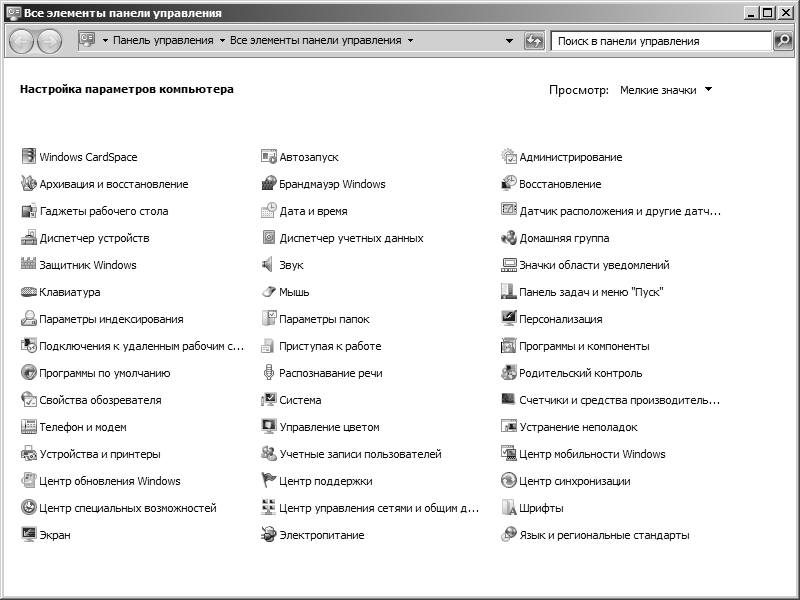
\includegraphics[height = 12\baselineskip]{./assets/y03s01-syssoft-lab-01-scr-01-controlpanel-bw.png}
				\caption{Панель керування Windows~7}
				\label{fig:01-win7-control-panel}
			\end{figure}
			
			Панель керування операційної системи Windows~7 надає виключно графічний інтерфейс налаштувань, і представляє не всі утиліти контролю, доступні в операційній системі. Для контролю апаратного забезпечення в Панелі керування надаються такі утиліти:
			\begin{description}
				\item [Адміністрування] Директорія, що~містить посилання на~більшість вбудованих засобів управління апаратним та~програмним забезпеченням операційної системи, розрахованих на~досвідчених користувачів та~системних адміністраторів. До~таких засобів належать: Конфігурація системи, Монітор ресурсів, Оптимізація дисків, Очистка дисків, Засіб перевірки пам\-'я\-ті Windows, Управління комп\-'ю\-те\-ром тощо.
				\item [Датчик місцезнаходження та~інші датчики] Розділ для~керування встановленими \allcaps{GPS} та~іншими датчиками.
				\item [Диспетчер пристроїв] Утиліта, яка дає можливість переглядати список пристроїв, підключених до~ком\-п'\-ю\-те\-ра, детальні відомості про~них, шукати, оновлювати та~видаляти їх~драйвери, управляти пристроями тощо.
				\item [Звук] Вікно для~керування звуковими пристроями, підключеними до~ком\-п'\-ю\-те\-ра: динаміками, навушниками, мікрофонами тощо. Керування здійснюється за~допомогою спливаючих вікон, у~яких можна обрати пристрій та~налаштувати його за~допомогою слайдерів (рівень гучності, підсилення, пониження шуму), випадаючих меню та~інших графічних елементів.
				\item [Клавіатура] Вікно для~управління налаштуваннями клавіатури та~вводом з~неї. Дозволяє налаштувати швидкість повтору вводу клавіш, переглянути детальну інформацію про підключену клавіатуру, оновити її драйвер.
				\item [Миша] Вікно для~управління налаштуваннями миші та~вводом з~неї. Дозволяє змінити функції клавіш та параметри прокрутки підключеного пристрою, переглянути дані про нього, оновити та видалити драйвер.
				\item [Система] Розділ перегляду базових відомостей про~систему та~її апаратне забезпечення. Дозволяє перейти до~більш спеціалізованих дій за~допомогою посилань у~боковому меню: переглянути детальнішу інформацію за~допомогою Диспетчера пристроїв та~змінити налаштування у~Додаткових параметрах системи.
				\item [Телефон і модем] Вікно для~створення та~управління мережевими підключеннями за~допомогою телефону або~модему.
				\item [Пристрої та принтери] Розділ, що~містить перелік деяких мультимедійних, мережевих та~пристроїв вводу, який дозволяє перейти до~їх налаштувань подвійним натисканням лівої кнопки миші.
				\item [Екран] Розділ налаштування параметрів підключених екранів та~зображення, що~виводиться на~них. 
				\item [Електроживлення] Розділ налаштування параметрів електроживлення та~заощадження електроенергії за~допомогою профілів живлення.
			\end{description}

		\subsection{Програма \allcaps{AIDA64}}
			Розглядаємо програму~\allcaps{AIDA64}~Extreme~(рис.~\ref{fig:02-aida64}). \allcaps{AIDA64}~Extreme~— це інструмент для перегляду детальної інформації про систему, її апаратне та програмне забезпечення, виявлення її недоліків та несправностей, а також оцінки її швидкодії, розроблений компанією FinalWire~Ltd.

			\begin{figure}[!htbp]
				\centering
				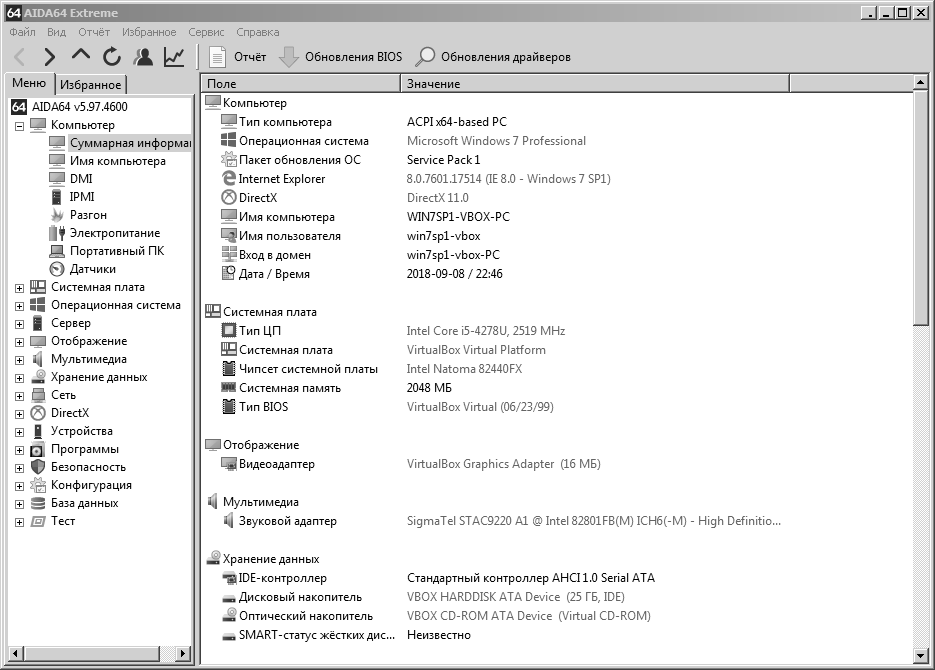
\includegraphics[height = 12\baselineskip]{./assets/y03s01-syssoft-lab-01-scr-02-aida64-bw.png}
				\caption{Вікно сумарної інформації про комп'ютер у~програмі \allcaps{AIDA64} Extreme}
				\label{fig:02-aida64}
			\end{figure}

			 Перегляд інформації про систему організований за допомогою бокового меню, яке містить вкладки, що відповідають властивостям та параметрам апаратного або програмного забезпечення.

			Виявлення недоліків та несправностей системи можливе за допомогою інструментів стрес-тестування, доступних у програмі, які використовують значне синтетичне навантаження, щоб користувач міг перевірити поведінку системи в екстремальних умовах.

			Оцінка швидкодії системи виконується за~допомогою тестів, під час яких виконуються ресурсомісткі операції та~збираються дані про~продуктивність їх виконання. В~кінці тесту на~екран виводяться отримані результати та~порівняльні значення. У~програмі~\allcaps{AIDA64} представлені такі тести: читання та~запис в~оперативну пам'\-ять, копіювання з~кеш-пам'яті в~оперативну, створення \allcaps{ZIP}-архівів, побудова фракталів Жюліа та~Мандельброта.

		\subsection{Утиліти \progname{msinfo32}, \progname{sc.exe}}
			Розглядаємо утиліти \progname{msinfo32}, \progname{sc.exe}. Утиліта~\progname{msinfo32}~(рис.~\ref{fig:03-msinfo})~— інструмент, вбудований в~операційну систему Microsoft Windows, який дозволяє переглядати детальну інформацію про її конфігурацію, включаючи інформацію про апаратне і~програмне забезпечення, а~також деякі існуючі налаштування. Навігація програмою виконується за допомогою бокового меню, яке містить дерево категорій, доступних для перегляду. У правій частині вікна виводиться зміст категорії, включаючи параметри та їх значення.
			Програма \texttt{msinfo32} дозволяє переглядати інформацію про~апаратні ресурси: номери переривань, зарезервовані адреси пам'яті тощо. Також можна переглянути список встановлених компонентів (пристроїв, аудіо- та~відеокодеків, неправильно встановлених пристроїв) і~детальну інформацію про~них. Інформація про~програмне забезпечення включає список системних драйверів, перелік змінних середовища та~їх значень, завдання для~принтерів, мережеві підключення та~інше.

			\begin{figure}[!htb]
				\centering
				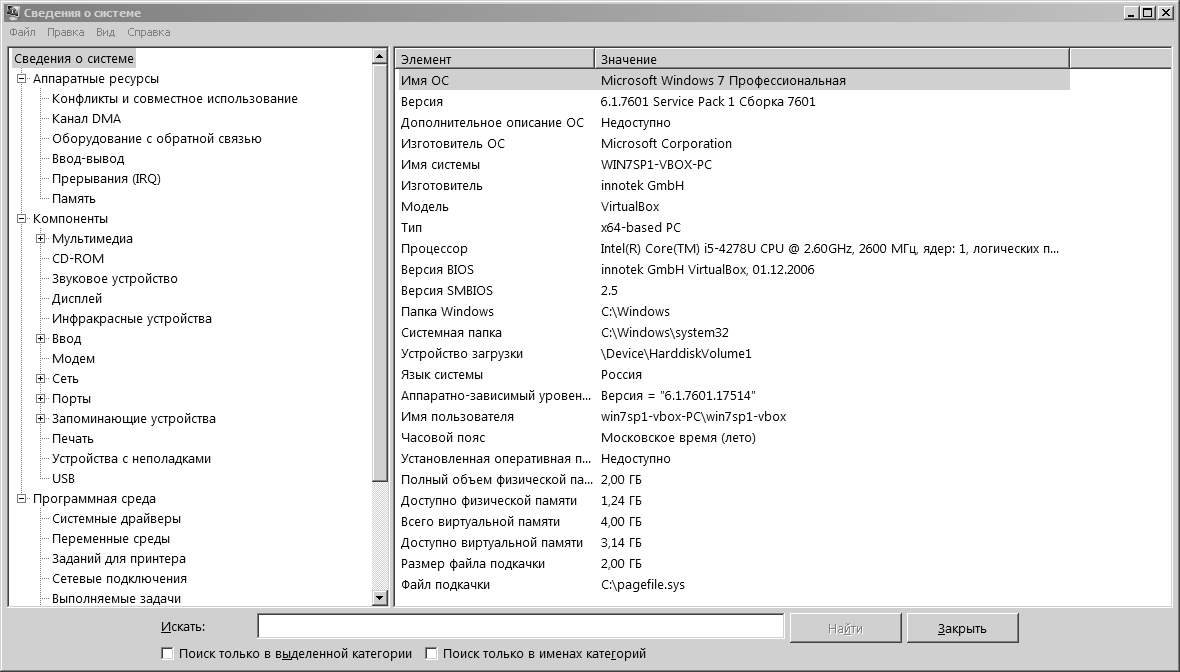
\includegraphics[height = 12\baselineskip]{./assets/y03s01-syssoft-lab-01-scr-03-msinfo-bw.png}
				\caption{Вікно утиліти~\progname{msinfo32}}
				\label{fig:03-msinfo}
			\end{figure}
			
			Утиліта \progname{sc.exe}~(Service Control, рис.~\ref{fig:04-scexe})~— це програма командного рядка, вбудована в~операційну систему Microsoft Windows, для~управління сервісами операційної системи.

			\begin{figure}[!htb]
				\centering
				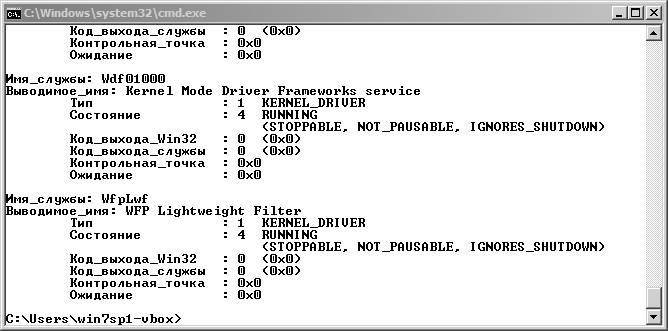
\includegraphics[height = 6\baselineskip]{./assets/y03s01-syssoft-lab-01-scr-04-scexe-bw.png}
				\caption{Вікно утиліти~\progname{sc.exe}}
				\label{fig:04-scexe}
			\end{figure}
			
			Однією з~можливостей програми є~запит статусу сервісів, який здійснюється за~допомогою параметра \texttt{query}. Наприклад, цей параметр можна використовувати для~перегляду встановлених та~активних драйверів.

		\subsection{Програма Driver Genius}
			Розглядаємо програму Driver Genius~(рис.~\ref{fig:05-driver-genius}). Driver Genius~— це програмний пакет для повного управління драйверами з можливістю автоматизації від компанії Driver-Soft.

			\begin{figure}[!htbp]
				\centering
				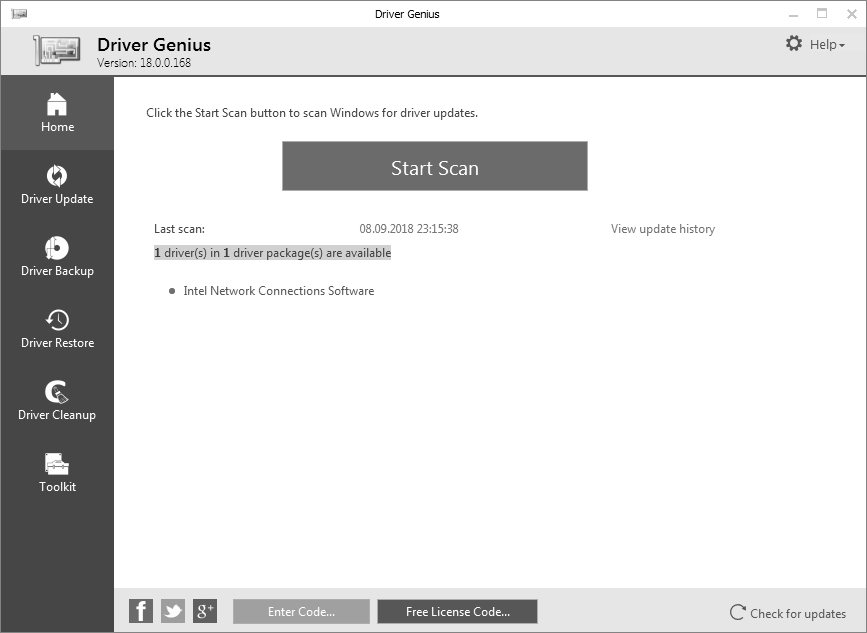
\includegraphics[height = 12\baselineskip]{./assets/y03s01-syssoft-lab-01-scr-05-drivergenius-bw.png}
				\caption{Головне вікно програми Driver Genius}
				\label{fig:05-driver-genius}
			\end{figure}

			Програма дає змогу шукати драйвери для підключених пристроїв у~мережі Інтернет, оновлювати існуючі драйвери, видаляти встановлені драйвери для~пристроїв, які не~застосовуються, створювати резервні копії встановлених драйверів тощо.

		\subsection{Порівняння програм AIDA64 і~Driver Genius}
			Програми \allcaps{AIDA64} та Driver Genius мають різні цілі: перша спрямована на аналіз та моніторинг системи, а друга~— на автоматичне управління драйверами. Незважаючи на різну спеціалізацію, програми мають схожі функції~(табл.~\ref{tab:01-aida64-driver-genius-comparison}).

			\begin{table}[!htbp]
				\centering
				\caption{Порівняння функцій програм \allcaps{AIDA64} Extreme та~Driver Genius}
				\label{tab:01-aida64-driver-genius-comparison}
				\begin{tabular}{
						v{6\gridunitwidth - 2\tabcolsep}
						n{3\gridunitwidth - 2\tabcolsep}
						n{3\gridunitwidth - 2\tabcolsep}
					}
						\toprule
							Функція & \allcaps{AIDA64} Extreme & Driver Genius\\
						\midrule
							Встановлення драйверів                             &            & \CheckMark \\
							Оновлення драйверів                                &            & \CheckMark \\
							Видалення драйверів                                &            & \CheckMark \\
							Резервне копіювання драйверів                      &            & \CheckMark \\
							Перегляд основних даних про~апаратне забезпечення  & \CheckMark & \CheckMark \\
							Перегляд детальних даних про~апаратне забезпечення & \CheckMark &            \\
							Перегляд даних про~програмне забезпечення          & \CheckMark &            \\
							Перегляд детальних даних про~мережу                          & \CheckMark &            \\
							Можливість моніторингу системи                     & \CheckMark &            \\
						\bottomrule
				\end{tabular}
			\end{table}

	\section{Висновок}
		Виконуючи дану лабораторну роботу ми ознайомились з~програмним забезпеченням для~контролю за~апаратурою комп'ютера та~автоматизованого керування драйверами. У~процесі лабораторної роботи були розглянуті як~вбудовані, так і~встановлювані інструменти. Рівень деталізації інформації у~вбудованих інструментах варіювався від~середнього до~високого в~залежності від~цільової доступності інструменту для~користувача: інструменти, представлені у~Панелі керування, зазвичай надавали поверхневу інформацію, а~для~отримання точніших даних потребували детальнішого розуміння роботи з~ними; інструменти, які~викликаються за~назвою програми, надавали дуже точний контроль та~інформацію для~адміністрування, однак, потребували чіткого розуміння процесу їх~роботи та~мали практичної користі для~звичайного користувача.
		
		Встановлювані інструменти~запропонували прийнятний баланс між~легкістю використання та~функціональністю: незважаючи на~інтуітивність процесу роботи з~ними, вони дозволяли з~легкістю виконувати завдання адміністрування, які~задовольнять більшість досвідчених користувачів та~системних адміністраторів.

		Програми \allcaps{AIDA64} Extreme і~Driver Genius виконують різні функції, однак обидві дозволяють переглядати основну інформацію про~систему. \allcaps{AIDA64} також може надавати детальнішу інформацію за~бажанням користувача, а~також дає можливість виконувати стрес-тестування та~моніторинг системи. У~свою чергу програма Driver Genius спрямована на~автоматичне керування драйверами, тому надає більше можливостей для~цього: пошук, встановлення, оновлення та~резервне копіювання драйверів з~можливістю відновлення. В~цілому, програми третіх сторін пропонують зручніший і~водночас детальніший інтерфейс для~складніших операцій порівняно з~системними.

\end{document}
